
\section{Loss functions}
\label{section:RelatedWork:Loss}

The loss function is critical in order to assess the error of a deep learning model.
Different loss functions, such as those defined in \Cref{section:BT:Loss},
are commonly used as a performance metric in artificial intelligence.
Dependent on the application of the machine learning problem, different loss functions suit different use-cases.

In order to find a proper loss function for our problem, we need to assess other loss functions as well.
This section will focus on a few specialized loss functions specifically designed to work well with extreme values, such as those we might encounter in our problem.

\subsection{DILATE}

% Time and shape distortion
Both MAE and MSE are proven to be robust loss functions for regular regression problems,
but a paper published by \citeauthor{Guen2019} highlights some problems when the shape of the target function matters
such as in time series.
\Cref{fig:dilate} shows three different fits to the same target function that all have
the same MSE error.

\begin{figure}[h!]
  \centering
  \begin{subfigure}[b]{0.3\textwidth}
    \centering
    \caption{Non informative prediction}
    \label{fig:dilate-non-informative}
    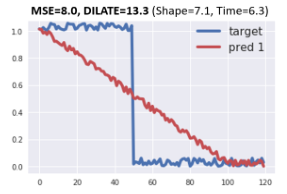
\includegraphics[width=\textwidth]{./figs/illustrations/dilate_ex1.png}
    \hfill
  \end{subfigure}

  \begin{subfigure}[b]{0.3\textwidth}
    \centering
    \caption{Correct shape, but with time delay}
    \label{fig:dilate-correct-shape}
    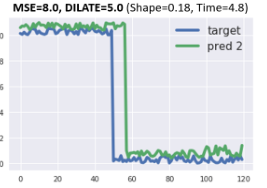
\includegraphics[width=\textwidth]{./figs/illustrations/dilate_ex2.png}
    \hfill
  \end{subfigure}
  \begin{subfigure}[b]{0.3\textwidth}
    \centering
    \caption{Correct time, but inaccurate shape}
    \label{fig:dilate-correct-time}
    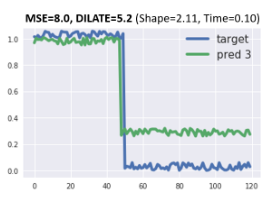
\includegraphics[width=\textwidth]{./figs/illustrations/dilate_ex3.png}
    \hfill
  \end{subfigure}
  \caption{Three examples of different shapes but same MSE error \citep{Guen2019}}
  \label{fig:dilate}
\end{figure}

In order to correct this problem, a new loss function is introduced, named 
\textbf{DILATE (Distrortion Loss including Shape and Time)} \cite{Guen2019}.
DILATE utilize a Neural Network method as an alternative to a mathematical function. 
It aims to accurately predict sudden changes and explicitly incorporates two terms
supporting precise shape and temporal change detection.

The paper concludes that DILATE is comparable to the standard MSE loss when evaluated on MSE,
and far better when evaluated on time and shape metrics.

The DILATE loss function does seem promising for the e-commerce problem space.
Predicting anomalies and their behavior is both a time-sensitive and shape-sensitive problem.
However, adding another neural network as a loss function could complicate an already complicated model even further.
Whether such a loss function is favorable to a standard loss function within the e-commerce domain remains to be seen,
but this is a problem space that could be favorable to explore further.

% Extreme value loss functions
\subsection{EVL}
\citeauthor{Ding2019} explores, in a 2019 paper, the weak performance of deep learning methods on real-world problems.
The inability of the methods to predict extreme values is presented as the leading argument for this.
This is argued as a result of the quadratic loss in the MSE loss function.

Taking inspiration from \textit{Extreme Value Theory} a new loss function is proposed.
The loss function, \textbf{Extreme Value Loss (EVL)},
employs a memory network in order to memorize extreme events in historical records.

\Cref{fig:evl} show two fitted time series from the results of the paper. They conclude
that the method is superior to the state-of-the-art methods in extreme event detection, and 
in time series prediction.

This loss function appears to address the predictive problem of forecasting anomalies,
something that could prove very useful.
It does, however, have a few drawbacks.
The increased complexity of the loss function would increase the computational complexity of a predictive framework.
Additionally, additional training data is needed for the training of the memory network,
making it less applicable in cases where there is not an abundance of data.

\begin{figure}[h!]
  \centering
  \begin{subfigure}[b]{0.5\textwidth}
    \centering
    \caption{Output from GRU}
    \label{fig:evl-example1}
    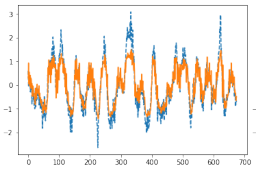
\includegraphics[width=\textwidth]{./figs/illustrations/evl_example1.png}
    \hfill
  \end{subfigure}

  \begin{subfigure}[b]{0.5\textwidth}
    \centering
    \caption{Output from EVL model}
    \label{fig:evl-example2}
    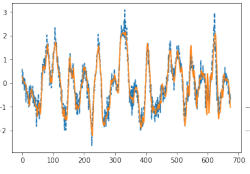
\includegraphics[width=\textwidth]{./figs/illustrations/evl_example2.png}
    \hfill
  \end{subfigure}
  \caption{Figures from \cite{Ding2019}}
  \label{fig:evl}
\end{figure}